\documentclass[border=3pt,tikz]{standalone}
\usepackage[utf8]{vietnam}
\usetikzlibrary{calc,angles,intersections,shapes.geometric,arrows,decorations.markings,arrows.meta,patterns.meta,patterns}
\usepackage{tikz-3dplot,pgfplots}
\pgfplotsset{compat=1.15}
\usepgfplotslibrary{polar}
\usepackage{amsmath}
\begin{document}
	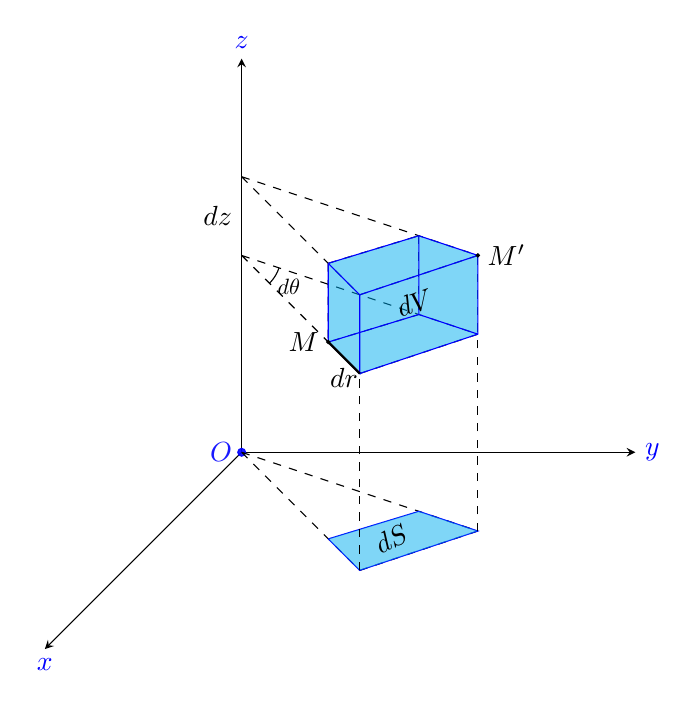
\begin{tikzpicture}[>=stealth]
	\draw[->] (0,0)--(5,0) node[right, blue] {$y$};
	\draw[->] (0,0)--(0,5) node[above, blue] {$z$};
	\draw[->] (0,0)--(-2.5,-2.5) node[below, blue] {$x$};
	\filldraw[blue, opacity=0.9] (0,0)circle(0.05) node[left] {$O$};
	\draw[dashed] (0,3.5)--(1.5,2) (0,3.5)--(3,2.5)--(1.5,2);
	\coordinate(u) at (1.1,2.4);
	\coordinate(k) at(2.25,2.75);
	\draw[dashed] (u)--(k);
	\begin{scope}[shift={(0,-3.5)}]
		\draw[dashed] (0,3.5)--(1.5,2) (0,3.5)--(3,2.5)--(1.5,2);
		\coordinate(m) at (1.5,2);
		\coordinate(n) at (3,2.5);
		\coordinate(e) at(2.25,2.75);
		\coordinate(w) at (1.1,2.4);
		\draw[blue] (w)--(e)--(n)--(m)--(w);
		\fill[cyan, opacity=0.5] (w)--(e)--(n)--(m)--(w);
		\node[rotate=27] at (1.9,2.4) {$dS$};
	\end{scope}
	\draw[dashed] (m)--(1.5,2) (n)--(3,2.5);
	\begin{scope}[shift={(0,-1)}]
		\draw[dashed] (0,3.5)--(1.5,2) (0,3.5)--(3,2.5)--(1.5,2);
		\coordinate(b) at (3,2.5);
		\coordinate(p) at (0,3.5);
		\coordinate(f) at (1.1,2.4);
		\coordinate(h) at (1.5,2);
		\coordinate(r) at (2.25,2.75);
		\coordinate(o) at (0,3.5);
		\draw[dashed] (u)--(1.1,2.4)--(2.25,2.75);
		\pic[ draw,inner sep=1pt, circle,black, draw,angle
		eccentricity=1.5, angle radius = 5mm] {angle = h--o--b};
		\node[black, above=0.08, scale=0.8] at (0.6,2.9) {$d\theta$};
	\end{scope}
	\draw[black] (p)--(0,3.5) node[left, midway] {$dz$};
	\draw[dashed] (k)--(r);
	\fill[cyan, opacity=0.5] (u)--(f)--(h)--(1.5,2);
	\fill[cyan, opacity=0.5] (1.5,2)--(3,2.5)--(2.25,2.75)--(u);
	\fill[cyan, opacity=0.5] (b)--(h)--(1.5,2)--(3,2.5);
	\draw[blue](u)--(f)--(h)--(1.5,2)--(u) (1.5,2)--(3,2.5)--(2.25,2.75)--(u) (3,2.5)--(b)--(h);
	\draw[blue] (k)--(r)--(b) (r)--(f);
	\filldraw[black] (f)circle(0.02) node[left] {$M$};
	\filldraw[black] (3,2.5)circle(0.02) node[right] {$M'$};
	\draw[black, thick] (f)--(h) node[midway, below] {$dr$};
	\node[rotate=20, black] at (2.2,1.9) {$dV$};
\end{tikzpicture}

And here's a new figure but this time I used tikz-3dplot :

\tdplotsetmaincoords{70}{110}
\begin{tikzpicture}[scale=5,tdplot_main_coords,>=stealth]
	\newcommand{\ptcyl}[3]{{#1*cos(#2)},{#1*sin(#2)},{#3}}
	% axis
	\draw[thick,->] (0,0,0) -- (1,0,0) node[anchor=north east]{$x$};
	\draw[thick,->] (0,0,0) -- (0,1,0) node[anchor=north west]{$y$};
	\draw[thick,->] (0,0,0) -- (0,0,1) node[anchor=south]{$z$};
	\coordinate (O) at (0,0,0);
	\coordinate (A) at (\ptcyl{0.6}{55}{0.6});
	\coordinate (B) at (\ptcyl{0.8}{55}{0.6});
	\coordinate (C) at (\ptcyl{0.8}{70}{0.6});
	\coordinate (D) at (\ptcyl{0.6}{70}{0.6});
	\coordinate (E) at (\ptcyl{0.6}{55}{0.8});
	\coordinate (F) at (\ptcyl{0.8}{55}{0.8});
	\coordinate (G) at (\ptcyl{0.8}{70}{0.8});
	\coordinate (H) at (\ptcyl{0.6}{70}{0.8});
	% Projections of points A, B & C
	\coordinate (I) at (\ptcyl{0.6}{55}{0});
	\coordinate (J) at (\ptcyl{0.8}{55}{0});
	\coordinate (K) at (\ptcyl{0.8}{70}{0});
	%THE ARCS
	\coordinate (M) at (0,0,0.6) ;
	\tdplotsetrotatedcoordsorigin{(M)}
	\tdplotdrawarc[tdplot_rotated_coords,thick,dashed]{(M)}{0.6}{55}{70}{}{}
	\tdplotdrawarc[tdplot_rotated_coords,thick]{(M)}{0.8}{55}{70}{}{}
	% arcs above
	\coordinate (N) at (0,0,0.9) ;
	\tdplotsetrotatedcoordsorigin{(N)}
	\tdplotdrawarc[tdplot_rotated_coords,thick]{(N)}{0.6}{55}{70}{}{}
	\tdplotdrawarc[tdplot_rotated_coords,thick]{(N)}{0.8}{55}{70}{}{}
	% arcs below
	\tdplotsetrotatedcoordsorigin{(O)}
	\tdplotdrawarc[tdplot_rotated_coords,thick,dashed,blue]{(O)}{0.6}{55}{70}{}{}
	\tdplotdrawarc[tdplot_rotated_coords,thick,dashed,blue]{(O)}{0.8}{55}{70}{}{}
	\tdplotdrawarc[tdplot_rotated_coords,thick,blue,->]{(O)}{0.18}{0}{55}{anchor=north}{$\theta$};
	\tdplotdrawarc[tdplot_rotated_coords,thick,blue,->]{(O)}{0.4}{55}{70}{}{};
	\draw (0.21,0.4,0) node [blue,scale=0.8] {$d\theta$};
	% Projections of points
	\draw [blue,thick] (O) -- (J) ;
	\draw [blue,thick,dashed] (O) -- (K) ;
	\draw [blue,thick,dashed] (A) -- (I) ;
	\draw [blue,thick,dashed] (B) -- (J) ;
	\draw [blue,thick,dashed] (C) -- (K) ;
	\draw [blue,thick,dashed] (A) -- (M) -- (D) ;
	\draw [blue,thick,dashed] (E) -- (N) -- (H) ;
	%the cube
	\draw [thick] (A) -- (E) -- (F) -- (B) -- (A) ;
	\draw [thick] (H) -- (G) -- (C) ;
	\draw [thick,dashed] (H) -- (D) -- (C) ;
	% points M & M'
	\draw [] (A) node {\textbullet} node [below left] {$M$};
	\draw [] (G) node {\textbullet} node [above right] {$M'$};
	% Names of the components
	\draw (0,0,0.7) node [left] {$dz$} ;
	\draw (\ptcyl{0.3}{45}{0}) node [] {$r$} ;
	\draw (\ptcyl{0.7}{50}{0}) node [] {$dr$} ;
	\draw (\ptcyl{0.8}{70}{0.3}) node [right] {$z$} ;
	\draw [thick,<-] (\ptcyl{0.8}{70}{0.7}) to [bend left] (\ptcyl{1}{70}{0.65}) node [below] {$dz$};
	\draw [thick,<-] (\ptcyl{0.7}{70}{0.8}) to [bend left] (\ptcyl{0.7}{90}{0.85}) node [right] {$dr$};
	\draw [thick,<-] (\ptcyl{0.6}{62.5}{0.8}) to [bend left] (\ptcyl{0.55}{90}{0.9}) node [right] {$r\ d\theta$};
\end{tikzpicture}
\end{document}